\documentclass[10pt,a4paper]{article}
\usepackage[latin1]{inputenc}
\usepackage[margin=1in]{geometry}
\usepackage{amsmath}
\usepackage{amsfonts}
\usepackage{amssymb}
\usepackage{graphicx}
\usepackage{booktabs}
\usepackage{gensymb}
\begin{document}
	
\section{Data Acquisition System(DAQ)(Outline)}

\subsection{Design}
\par Rockets, by their very nature, are very complicated systems to tackle and have work consistently and safely. There are many variables involved in the problem of rockets, which creates many obstacles on the road from design to launch. To help us better fill in the blank spaces that need to be filled, we test our systems. The objective of these tests is data, which we can use to create more accurate models for actual launches.
\par Temperature data is major key. In our static test cell, we currently capture temperatures in the plumbing, on the outside of the combustion chamber, and on the outside of the nozzle. Combined with ambient temperature data collected at a control distance away from the test area, this gives a good example of what the behavior of our engine is in terms of temperature.
\par Another important aspect of data that we collect is pressure. Our current setup collects pressure at two points, the plumbing and the combustion chamber. The plumbing tells the pressure in the run tank, which we use to realize our pressure at the point where we are ready to ignite the engine. The combustion chamber pressure, with the plumbing pressure data gives us a differential that we can then use to calculate our pressure-based thrust. 
\par Lastly, we have a load cell fastened to the top of our rig, which captures our raw thrust when the engine is ignited. Our current rig setup is also optimized to reduce friction and gather the cleanest numbers. To summarize, all of our data is integral to our rocket launches, from producing more accurate models to assessing the safety factors of our systems.

\par The current hardware systems used in our DAQ infrastructure are load cells, pressure transducers, and thermocouples. To collect this information we use a 2 National Instruments DAQ Boards, a USB 6002, and USB 6009 model. These models are not optimized on their own to take raw voltages and turn them into usable data, several workarounds have been implemented to get accurate numbers. While the pressure transducers provide output voltages that are optimal for the NI boards, the load cell currently requires a TMO-2 Signal Conditioner to provide the correct excitation voltage to the sensor and properly erase the noise from the sensor. The thermocouples on their own are also not conducive to data collection, due to the fact that most thermocouples, including the K-types that we use, output a very small voltage, on the order of about ~5mV at ambient temperature. To rectify this, a circuit with amplifiers that adjust the signals from the temperature sensors is used such that the voltages at ambient are closer tp ~1.5V.
\par All of our sensors are currently connected in differential configurations, without ground connections. The purpose of this is to further reduce the noise seen in the data collection software, and increase the accuracy of the readings. Past the sensors, connections, amplifiers, and NI boards, the end of the line for the path the data flows down is the computers. Both NI boards connect to a Dell PC that is located within the test cell adjacent to the testing rig, and then connected via Ethernet cable to the control room. From the control room, a secondary computer can be used to access the pc in the test cell via remote desktop connection. This is where the NIMax and LabView softwares are accessed and used when tests are conducted in the test cell.


\par Grand Schematic (Has not been made yet)

\par After the sensors has transmitted the voltages through the NI boards to be processed, several things must be done to turn these into workable data to create valid models for future tests and launches. Using software is a very robust and efficient way of managing the numbers. For the purposes of the rocket, two specific National Instrument softwares are used. The first being NIMax, which manages and records the data from the NI boards. The second being LabView, where a Graphical User Interface(GUI) has been written using block diagram components to show real time data during tests, and record them for post-processing. 
\par Both software programs are necessary to be in use during a test, and are interwoven in their necessity. Currently, the LabView program will only run correctly if the NIMax is set up properly as well. NIMax requires the DAQ boards to be properly connected to the computer, and then a task created and specified back in the LabView. Two tasks have to be created and used at the same time, because we are using two NI boards. One for the load cell and pressure transducers, and another for the thermocouples. Once these tasks have been confirmed to be acquiring data, the LabView program then reads the data from the boards and outputs the data both into a graphical form for the real-time analysis during a test, and into .csv files with the location pre-specified for post-processing.
\newpage
\begin{figure}[h!]
	\centering
	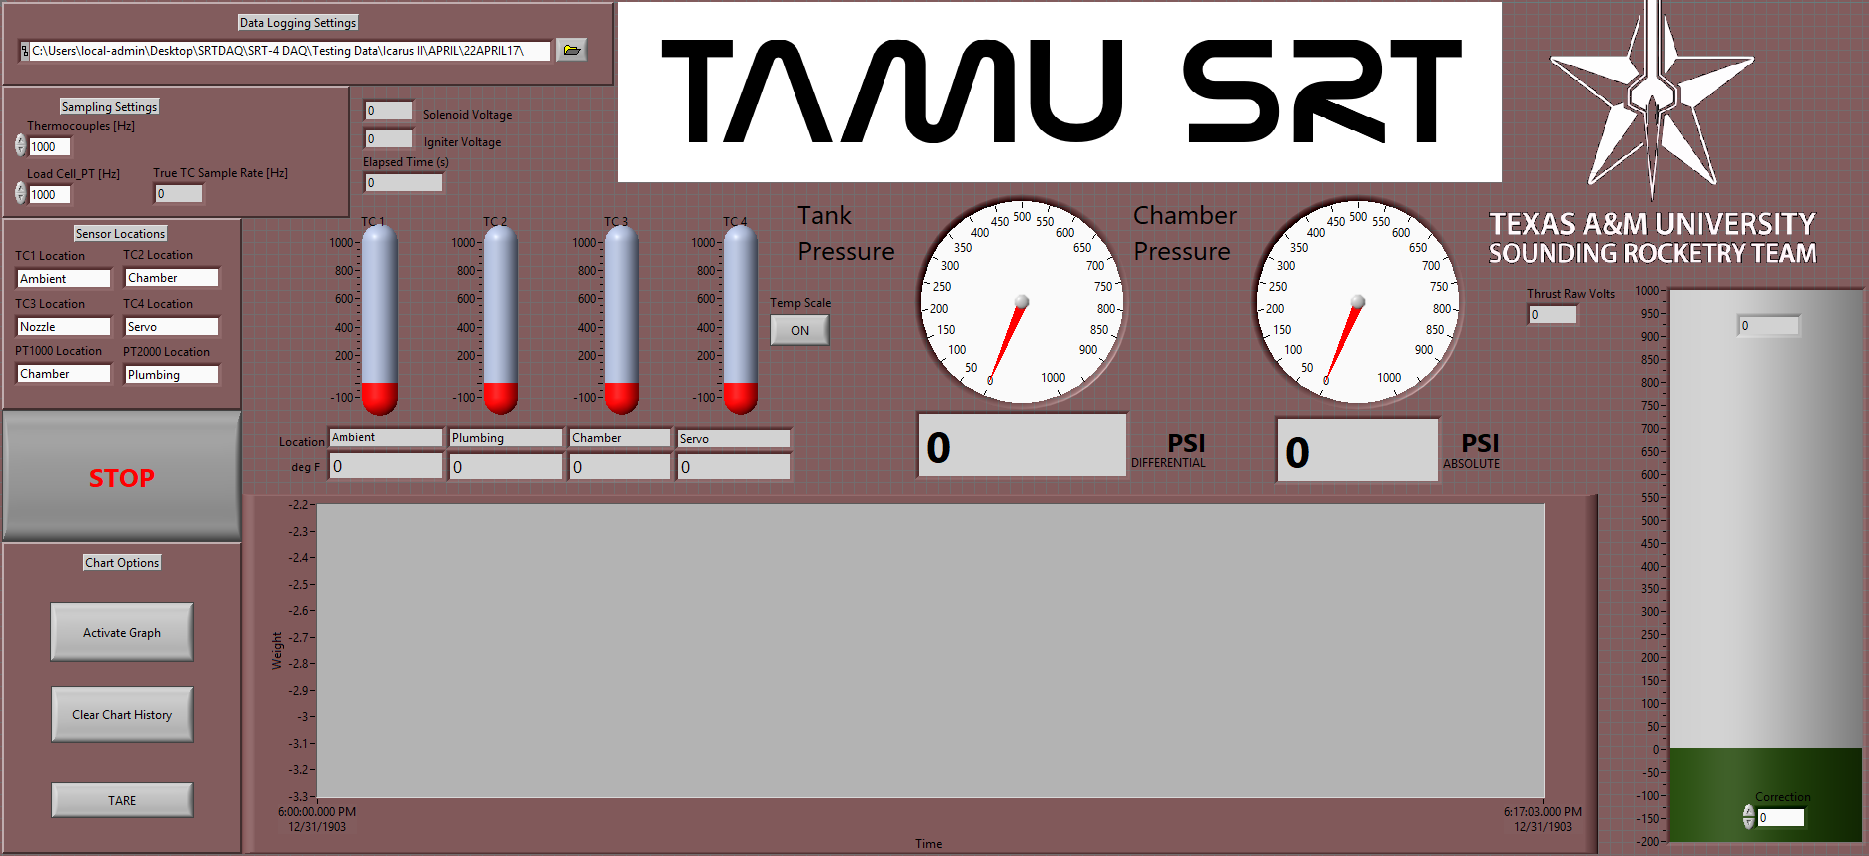
\includegraphics[width=1\textwidth,keepaspectratio]{./figs/LVGUI.png}
	\caption{LabView GUI}
	\label{fig:This is a placeholder}
\end{figure}



\newcommand{\ra}[1]{\renewcommand{\arraystretch}{#1}}
\begin{table*}\centering
	\ra{1.3}
	\begin{tabular}{@{}ccccccc@{}}\toprule
		& \multicolumn{2}{c}{Load Cell} & \phantom{abc}& \multicolumn{3}{c}{Pressure Transducers}\\
		\cmidrule{1-3} \cmidrule{4-6}
		 &&Rated Output: $3mV/V$ &&& Rated Output: \\ &&Safe Temp. Range: -65$^{\circ}$ to 250$^{\circ}$F &&& Safe Temp. Range: \\ &&Excitation Voltage: 10 VDC &&& Excitation Voltage: \\ \midrule
		& \multicolumn{5}{c}{Thermocouples}\\
		\cmidrule{4-5}
		&&& Rated Output: \\ &&& Safe Temp. Range:\\ &&& Excitation Voltage: \\  \midrule \midrule
		& \multicolumn{4}{c}{DAQ NI Boards}\\ \midrule
		& \multicolumn{2}{c}{NI USB 6009} & \phantom{abc}& \multicolumn{3}{c}{NI USB 6002}\\
		\cmidrule{1-3} \cmidrule{4-6}
		&&Rated Output:&&& Rated Output: \\ &&Safe Temp. Range:  &&& Safe Temp. Range: \\ &&Excitation Voltage: &&& Excitation Voltage: \\
		\bottomrule
	\end{tabular}
	\caption{Hardware Specifications}
\end{table*}


\subsection{Manufacturing}

Circuit Diagram - Still needs to be finalized 
\begin{figure}[h!]
	\centering
	
\includegraphics[width=0.25\textwidth]{./figs/logo_srt.png}
	\caption{This is a placeholder}
	\label{fig:This is a placeholder}
\end{figure}
\newpage
\subsection{Testing}

\par One of the primary objectives of testing is the collection of sufficient adequate data during a rocket engine ignition test or a nitrous cold flow test in order to create better models of rocket performance and behavior. As mentioned earlier, post-processing is how most of this is achieved. The hardware section of this report details the components used to collect data, and briefly mentions the noise and error seen in the current configuration. Because the NI boards aren't made specifically for the purpose of collecting rocket engine data, there are some discrepancies propagated through the numbers. 
\par One specific example of this is of the thermocouples. Because they have such low output voltages, they produce a high amount of noise when input into the computers. The 6002 and 6009 NI boards do not have a high enough precision to correctly interpret this data. To compare, the NI USB 9211 has a range of (+/-) 80 mV where the NI USB 6002 (+/-) 10 V. Taking into account the typical voltage outputs of thermocouples being very low, the noise seen when the thermocouples are connected sans circuit is expected. 
\par The solution for the load cell signal discrepancies is using the TMO-2 signal conditioner. (Need more to talk about with the signal conditioner) Along with this, the load cell is calibrated before every test by adding weights, and then recording the voltages output by the load cell in the NIMax software. Putting this data in excel will produce a Force v Volt plot with a linear trend, the slope and y-intercept being input into the LabView code, and outputting corrected force measurements.


\end{document}